% !TEX root = ../main.tex
%
\chapter{Discussion}
\label{sec:discussion}

% TODO: Write discussion

% Interpretation of results in the context of existing NeRF creation methods
% Implications for the film and VFX industry
% Discussion on the integration of user feedback into the prototype
% Limitations of the study and the prototype

\section{Interpretation of Results}
\label{sec:discussion:results}

\section{Implications for the Film and VFX Industry}
\label{sec:discussion:implications}

\section{Integration of User Feedback}
\label{sec:discussion:user-feedback}

Based on the issues identified during user testing, several adjustments were made to enhance the usability and intuitiveness of the application. These changes are outlined below:

\paragraph{Improved Navigation}
To address the confusion in navigation to the dashboard (\ref{sec:results:issues:navigation}), a dedicated button was added to the navigation bar. 
This feature has should improved the clarity of  navigation to users significantly. \fref{fig:fix-1}

\begin{figure}[htb]
  \centering
	
\includegraphics[width=0.5\textwidth]{figures/fix-1.png}
	\caption{Dedicated Button for Dashboard Navigation}
  \label{fig:fix-1}
\end{figure}

\paragraph{Clarified Wording}
The wording on the button to start the training process was changed from \emph{"Start Processing"} to \emph{"Start Training"}, which aligns better with user expectations and reduces confusion. \fref{fig:fix-2}

\begin{figure}[htb]
	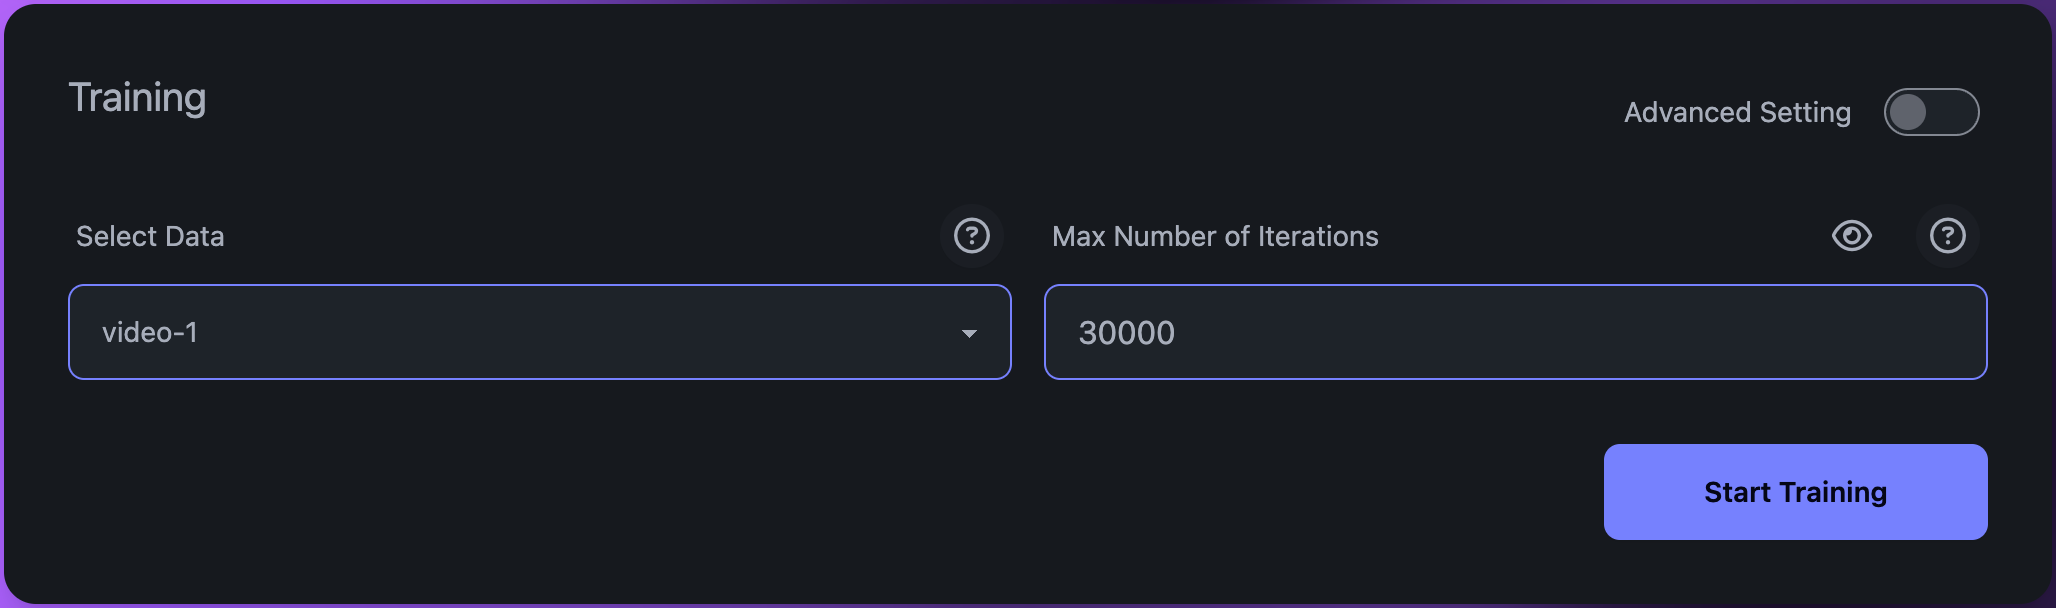
\includegraphics[width=\textwidth]{figures/fix-2.png}
	\caption{Consistent Wording for Training Button}
  \label{fig:fix-2}
\end{figure}

\paragraph{Enhanced Project Creation}
The project creation process was moved into a modal dialog, which not only eliminates a point of confusion but also clarified the need to name projects before creation. \fref{fig:fix-3}

\begin{figure}[htb]
	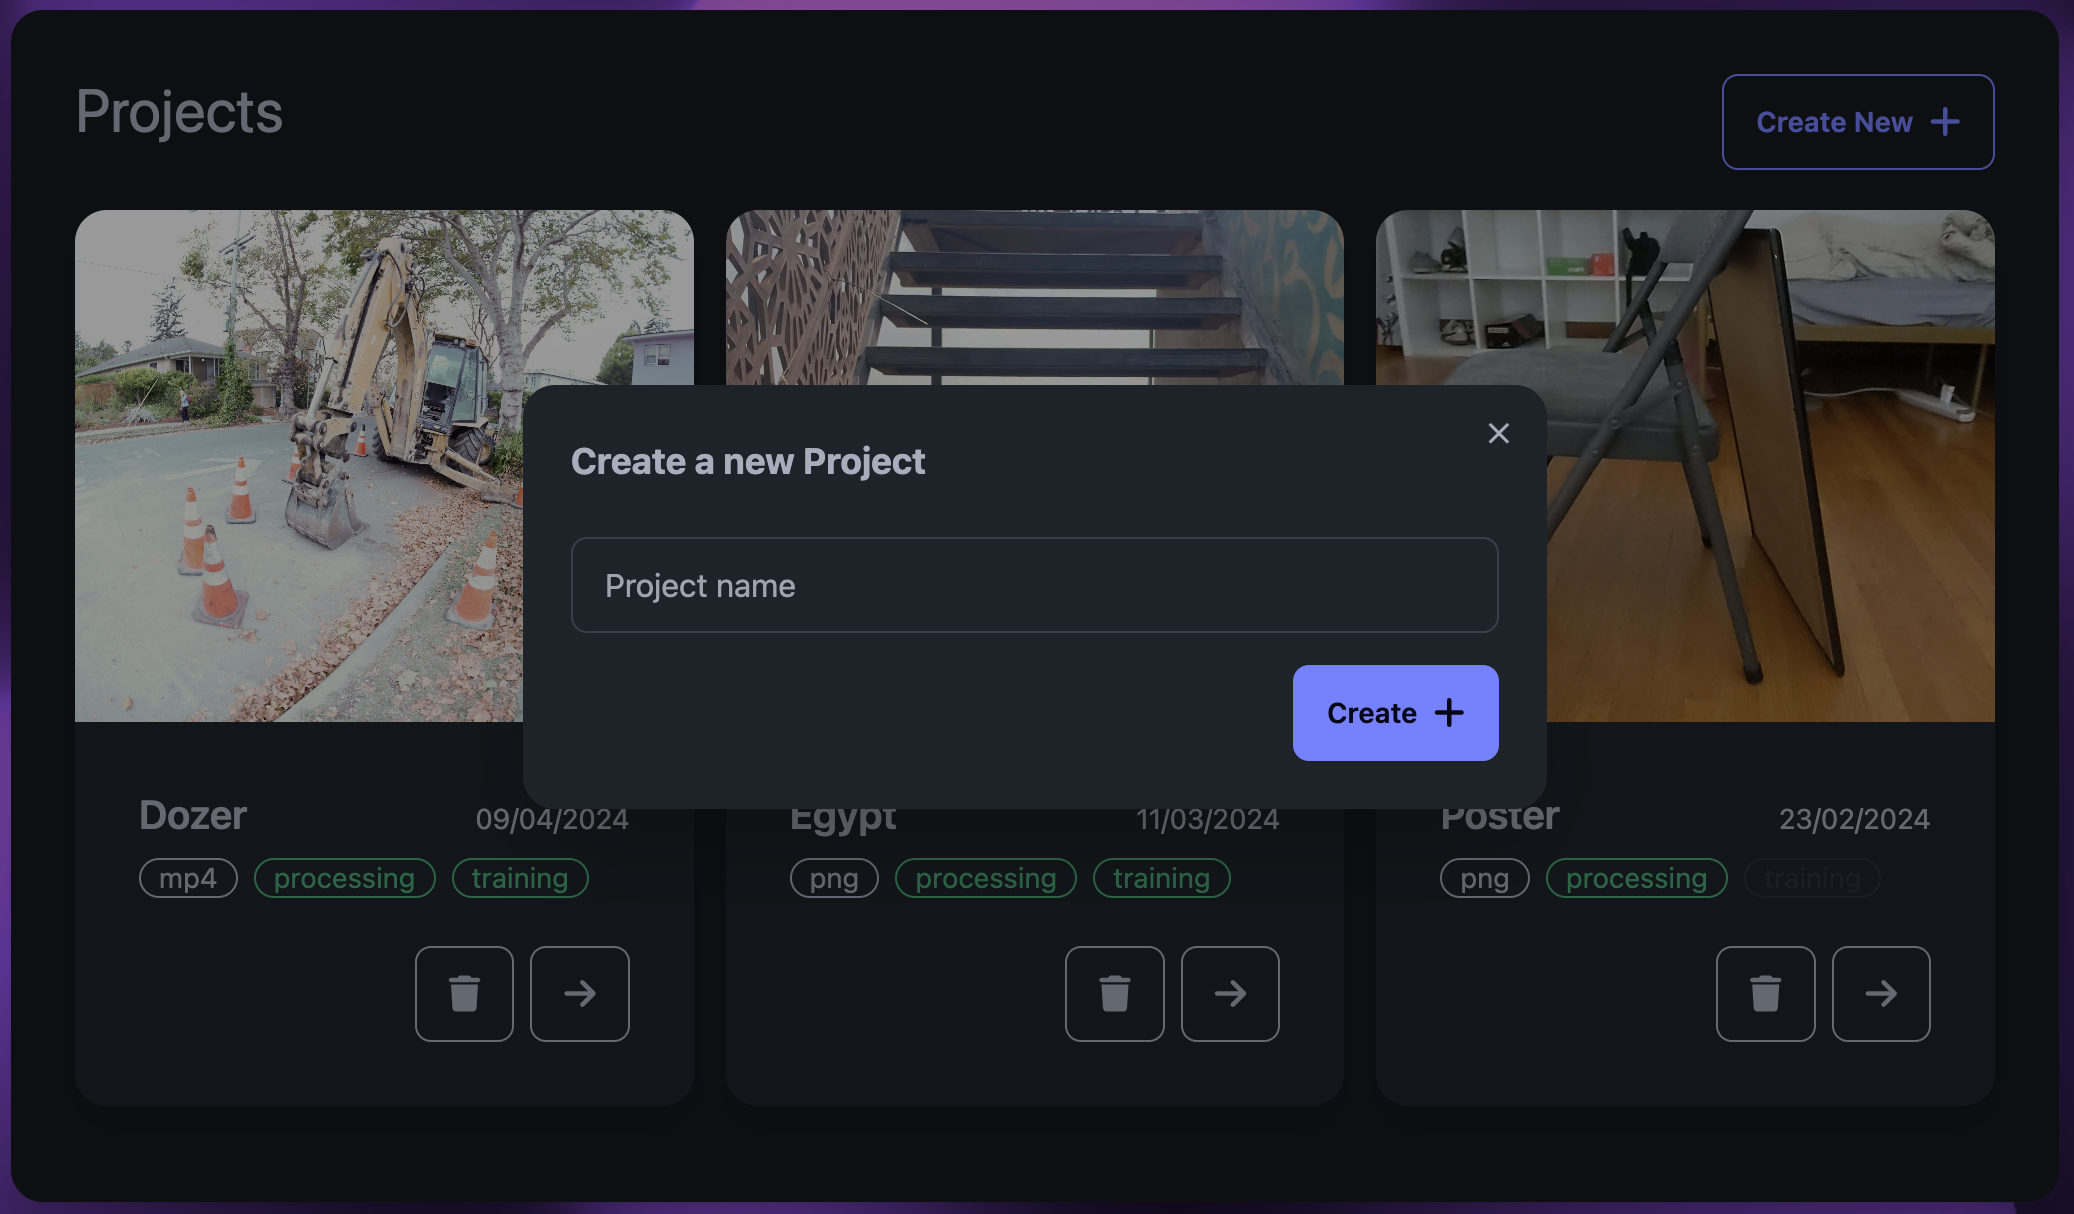
\includegraphics[width=\textwidth]{figures/fix-3.png}
	\caption{Modal Dialog for Project Creation}
  \label{fig:fix-3}
\end{figure}

\paragraph{File Upload Improvements}
The file upload process was improved by adding some guardrails, to ensure user would not accidentally skip a step. 
The upload button starts out disabled, so that the only interactive element is the file-input field.
Once a file is selected, the button becomes active, indicating to the user that they can proceed to upload their selected file.
Only one the file is uploaded, the UI elements related to pre-processing appear, guiding the user through the next steps. 
This solution is likely to prevent many of the issues users encountered when uploading files during testing. \fref{fig:fix-4}


\begin{figure}[htb]
  \begin{subfigure}{\textwidth}
    \centering
    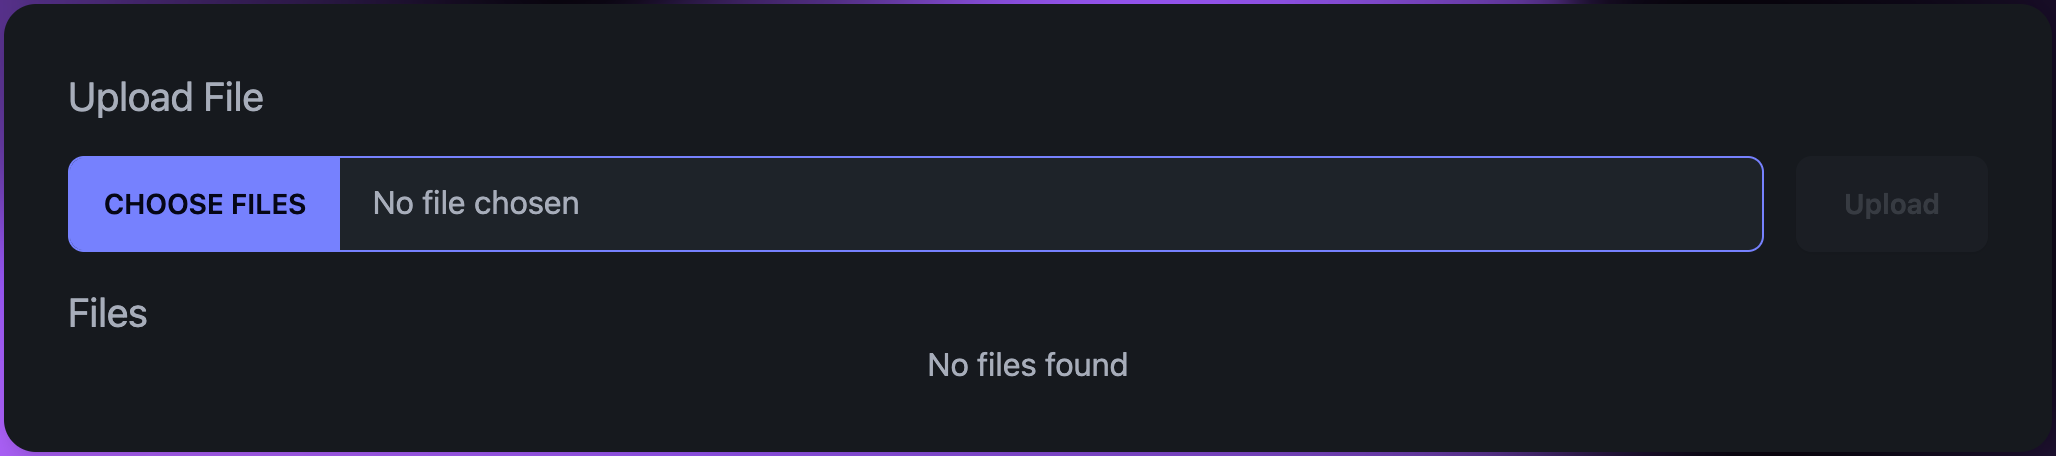
\includegraphics[width=.8\linewidth]{figures/fix-4.1.png}
    \caption{Initial State}
  \end{subfigure}
  \begin{subfigure}{\textwidth}
    \centering
    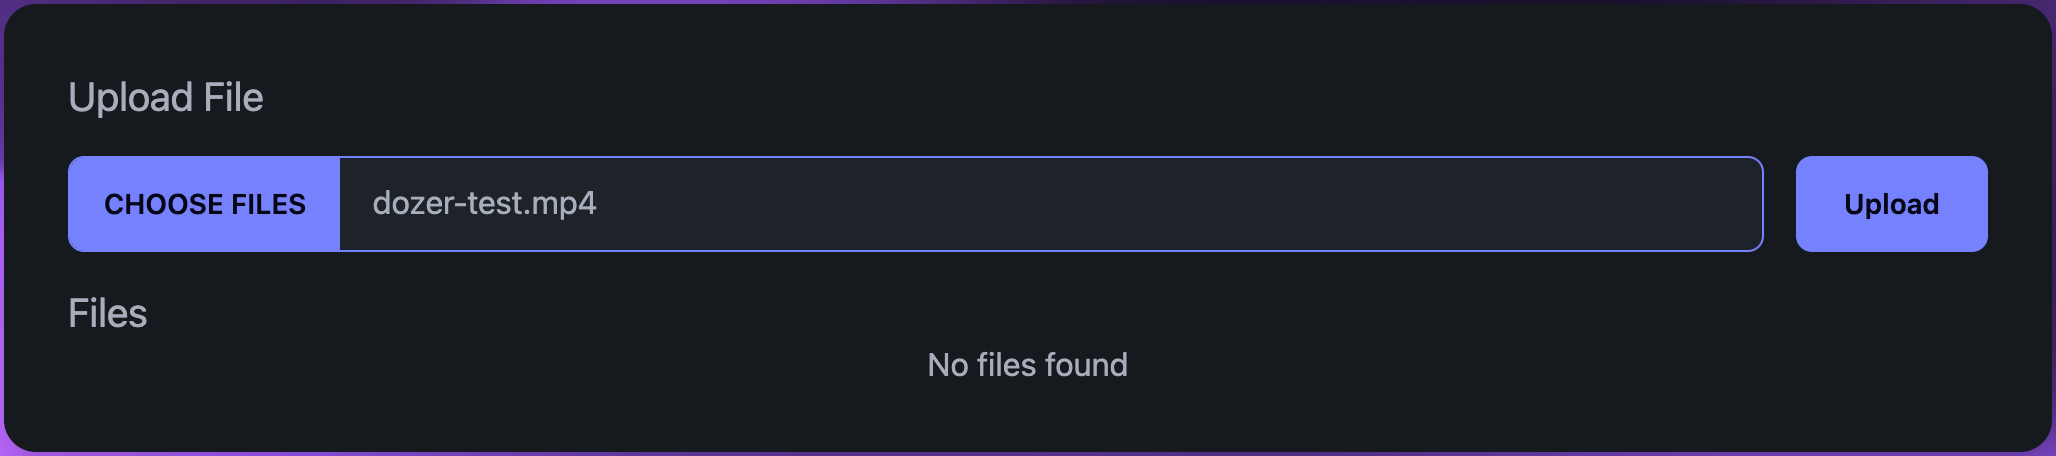
\includegraphics[width=.8\linewidth]{figures/fix-4.2.png}
    \caption{File Selected}
  \end{subfigure}
  \begin{subfigure}{\textwidth}
    \centering
    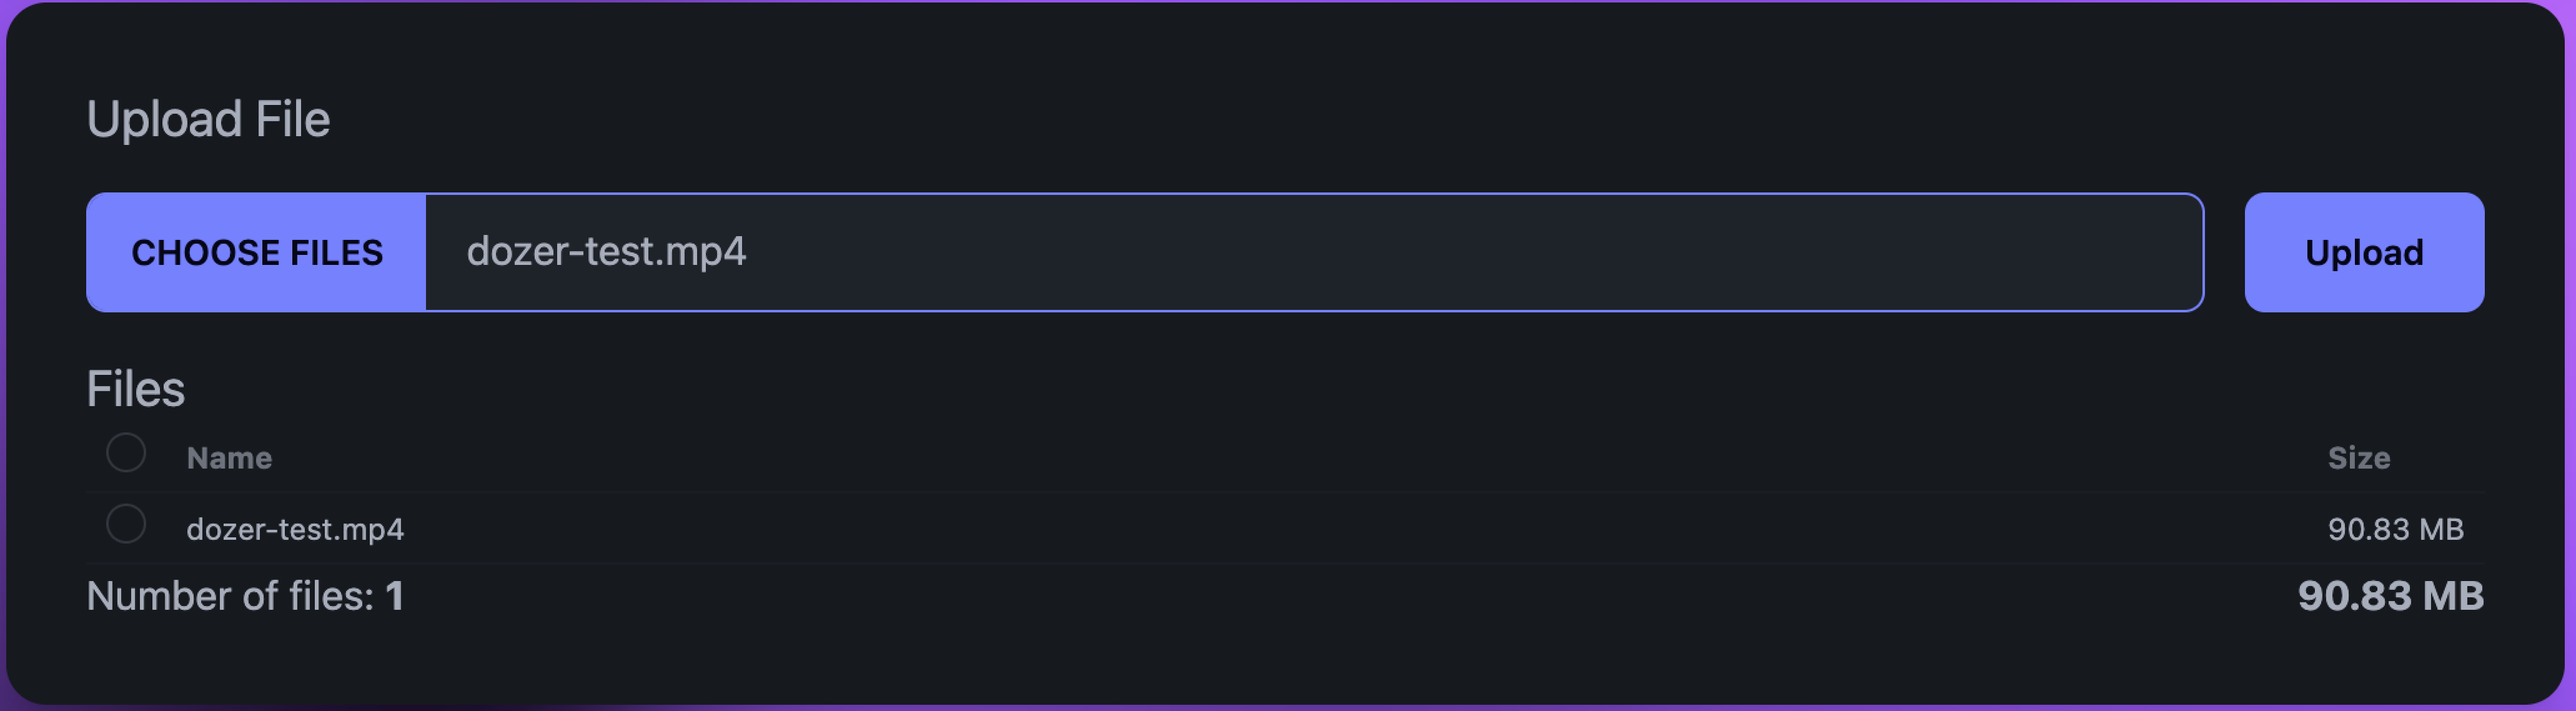
\includegraphics[width=.8\linewidth]{figures/fix-4.3.png}
    \caption{File Uploaded}
  \end{subfigure}
	\caption{Improved File Upload Process}
  \label{fig:fix-4}
\end{figure}

\section{Limitations}
\label{sec:discussion:limitations}
